\documentclass[11pt]{article}
\usepackage[margin=1in]{geometry}
\usepackage{amsmath,amssymb}
\usepackage{booktabs}
\usepackage{graphicx}
\usepackage{caption}
\usepackage{setspace}
\usepackage[hidelinks]{hyperref}
\onehalfspacing

\title{Does Compressing the Settlement Cycle Improve Market Quality?\\
\large Evidence from the 2024 US Move to T+1}
\author{Sean Qin \\ \small ECON 381-2, Northwestern University}
\date{June 2026}

\begin{document}
\maketitle

\begin{abstract}
\noindent On 28 May 2024 the United States shortened the standard equity settlement
cycle from two business days (T+2) to one (T+1). I estimate the effect on market
quality using a within-firm difference-in-differences design: for cross-listed
firms, the US-listed line moved to T+1 while the same firm's home-market line
remained on T+2, so the home line controls for fundamentals. In a panel of 19
cross-listed firms (38 listings; 7{,}184 listing-days, January--September 2024),
the bid--ask spread coefficient is statistically insignificant but imprecise: its 95\% confidence interval, roughly $[-0.56,\,0.58]$ in log points,
cannot rule out economically large changes in either direction, so I read it as no evidence of a transaction-cost effect rather than a tight zero. This
null is robust---it survives weekly aggregation and reappears in an independent
sample of non-cross-listed US versus European stocks that share no arbitrage book.
A volatility decline in the cross-listed sample ($-0.198$) fails a pre-period placebo and reverses sign in the non-cross-listed
sample, so I do not read it as causal. The contribution is a bounded null on transaction costs, along with two practical lessons: few-cluster inference can manufacture spurious significance, and placebo and alternative-control tests discipline causal claims.
\end{abstract}

\section{Introduction}
The settlement cycle---the lag between trade execution and the final exchange of
cash for securities---is basic market plumbing with first-order consequences for
counterparty risk, margin, and collateral. An unsettled trade exposes each side to
the risk that the other fails to deliver; a longer cycle therefore requires more
clearinghouse margin and ties up more collateral. Regulators argue that shortening
the cycle reduces systemic risk and frees capital, and after the meme-stock margin
disruptions of 2021 the SEC adopted amendments shortening the US cycle from T+2 to
T+1, effective 28 May 2024. Skeptics counter that compressing the operational
timetable raises settlement failures and, because the rest of the world stayed on
T+2 (the UK and EU target 2027), creates cross-border funding and FX misalignment.
Which view dominates is an empirical question, and because the 2024 change is so
recent, it has not yet been answered in the academic literature; industry and
exchange commentary (e.g.\ LSEG, ISDA) has discussed operational impacts but not
estimated causal effects on market quality.

The most closely related evidence is Baig et al.\ (2022), who study the 2017 US
move from T+3 to T+2 and find that liquidity improved. Their setting provides a difference-in-differences template around a known event date, but the 2024 episode differs because the US moved while comparable markets did not, creating a natural control group. For a firm
cross-listed in New York and London, the New York line settles T+1 after 28 May
2024 while the London line of \emph{the same firm} still settles T+2. Comparing the
two lines around the event isolates the settlement change from everything about the
firm itself.

\section{Econometric Model}
Let $Y_{it}$ be a market-quality outcome for listing $i$ on day $t$. Define
$\text{Treat}_i = 1$ for the US-listed line of each cross-listed pair and
$\text{Post}_t = 1$ on and after 28 May 2024. The main estimating equation is a
two-way fixed-effects difference-in-differences:
\begin{equation}
Y_{it} \;=\; \alpha_i \;+\; \delta_t \;+\; \beta\,(\text{Treat}_i \times \text{Post}_t) \;+\; \varepsilon_{it},
\label{eq:did}
\end{equation}
where $\alpha_i$ are listing fixed effects (absorbing time-invariant differences
between, e.g., the BP ADR and BP's London ordinaries), $\delta_t$ are date fixed
effects (absorbing market-wide shocks common to all listings on a day), and
$\beta$ is the coefficient of interest. Identification comes from comparing, within
a firm-day, the change in the US line to the change in its home line; the listing
fixed effects mean only the \emph{differential} movement at the event date
contributes to $\beta$. Standard errors are clustered by firm, since a firm's two
lines are mechanically correlated.\footnote{With only 19 firm clusters,
cluster-robust standard errors rest on large-$G$ asymptotics and can over-reject;
the standard remedy is the wild cluster bootstrap (Cameron, Gelbach \& Miller
2008). That estimator is outside this course's toolkit, so I report conventional
clustered standard errors and treat any marginal significance cautiously.} Because
all treated listings switch on the same date, this is an ordinary $2\times2$
design and the staggered-timing critique of Goodman-Bacon (2021) does not apply.

\paragraph{Interpreting $\beta$.}
Because treatment is defined \emph{within} cross-listed pairs, $\beta$ identifies
the effect on the US line relative to its home twin---a within-pair
differential, not the absolute effect of T+1 on US market quality. One threat is that arbitrageurs linking the two lines now face a T+1/T+2
settlement mismatch, so the ``control'' line could be partially affected too
(a SUTVA concern). If the mismatch raises frictions on both lines, the within-pair estimate understates the absolute
effect, and a within-pair null bounds the absolute effect rather than proving it
zero. Section~\ref{sec:robust} addresses this with a control group that
shares no arbitrage book.

\paragraph{Other identification concerns.} The identifying assumption is parallel
trends, tested with an event-study version of \eqref{eq:did} (leads should be
zero) and a pre-period placebo. US and European closing times differ, so a daily
$\delta_t$ pairs information sets that are one session apart; I address this with a
weekly-aggregation check. Levels differ across listing types (currency, tick
size); listing fixed effects absorb these, and only a differential change at the
event biases $\beta$.

\section{Data}
\textbf{Source and construction.} Daily open, high, low, close, and volume for each
listing come from Yahoo Finance for 2 January--30 September 2024. The sample is 19
firms cross-listed between a US exchange and a still-T+2 home market (London,
Frankfurt, Paris, Zurich)---e.g.\ Unilever (UL/ULVR.L), BP, Shell, AstraZeneca,
GSK, HSBC, Diageo, SAP, TotalEnergies, Novartis. An \textbf{observation} is a
listing-day: 38 listings $\times$ roughly 190 trading days $= 7{,}184$ after
dropping days with missing prices. I include every firm with both a US listing and a single home-market listing on a
still-T+2 exchange that traded continuously over the window; no firm is dropped on
the basis of its outcomes.

\textbf{Outcomes}, built from daily data, are: the Corwin--Schultz (2012) high--low
estimator of the bid--ask spread; the Amihud (2002) illiquidity ratio
$|r_{it}|/\text{dollar volume}_{it}$; Parkinson (1980) range volatility
$\sqrt{\ln(H/L)^2/(4\ln 2)}$; and turnover. All enter in logs. Because the spread is estimated from daily high-low data rather than observed quotes, the spread outcome is a noisy proxy for transaction costs; this likely contributes to the wide confidence intervals below.

\begin{table}[h]\centering
\caption{Descriptive statistics, pre-period (2 Jan--27 May 2024)}
\begin{tabular}{lcccccc}
\toprule
 & \multicolumn{3}{c}{Treated (US line)} & \multicolumn{3}{c}{Control (home line)} \\
\cmidrule(lr){2-4}\cmidrule(lr){5-7}
 & Mean & SD & Median & Mean & SD & Median \\
\midrule
CS spread            & 0.0030 & 0.0045 & 0.0000 & 0.0031 & 0.0045 & 0.0000 \\
Parkinson volatility & 0.0076 & 0.0035 & 0.0069 & 0.0104 & 0.0055 & 0.0093 \\
Daily return         & 0.0010 & 0.0144 & 0.0011 & 0.0010 & 0.0141 & 0.0008 \\
Volume (shares, m)   & 3.94   & 4.55   & 2.26   & 29.60  & 55.84  & 6.89   \\
Observations         & \multicolumn{3}{c}{1{,}919} & \multicolumn{3}{c}{1{,}919} \\
\bottomrule
\end{tabular}
\caption*{\footnotesize Spreads are balanced across groups pre-event; level
differences in volatility and volume across listing types are absorbed by listing
fixed effects. The zero median Corwin--Schultz spread reflects the estimator's
convention of truncating negative daily estimates to zero.}
\end{table}

\section{Results}
Before the regressions, Figure~\ref{fig:trends} plots the raw weekly mean spread for
treated and control listings. The two series move together both before and after
28 May 2024, with no visible break at the event.
(The formal parallel-trends test is the event study in Figure~\ref{fig:es}.)

\begin{figure}[h]\centering
\IfFileExists{trends_REAL.png}{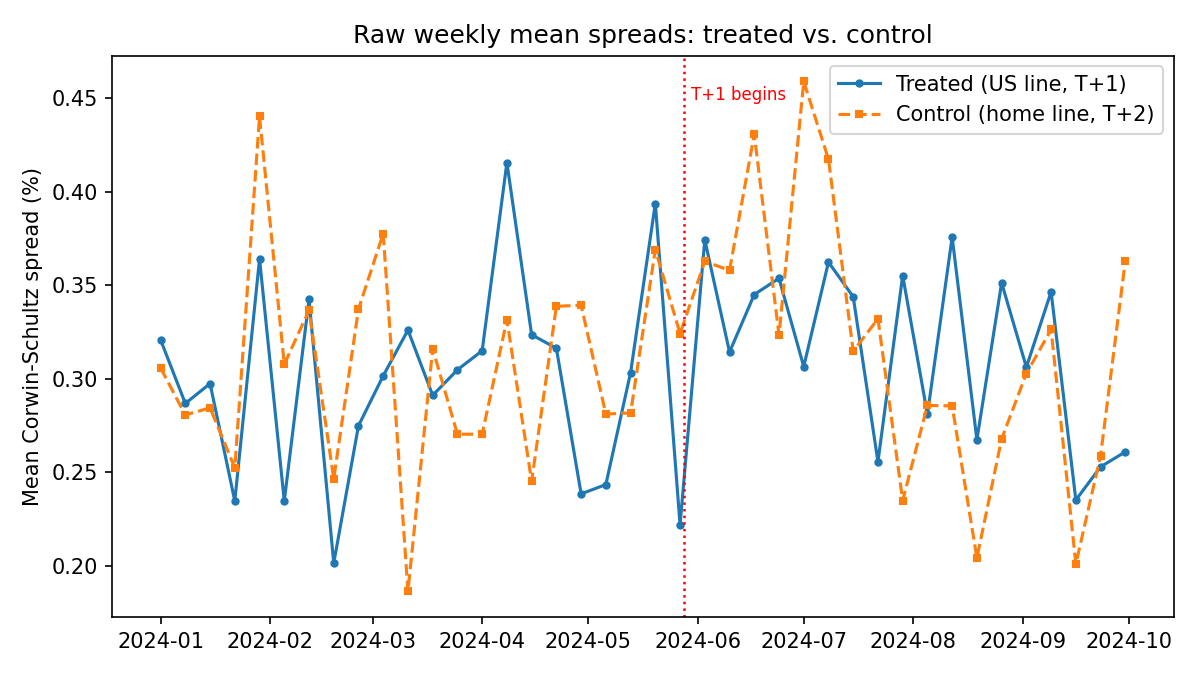
\includegraphics[width=.82\textwidth]{trends_REAL.png}}{\fbox{Upload trends\_REAL.png}}
\caption{Raw weekly mean Corwin--Schultz spreads (\%) for treated (US, T+1) and
control (home, T+2) listings; the dotted line marks 28 May 2024. The series track
each other across the event, consistent with the regression null.}
\label{fig:trends}
\end{figure}

Table~\ref{tab:main} reports $\beta$ from equation~\eqref{eq:did}.

\begin{table}[h]\centering
\caption{Effect of T+1 on market quality (within-firm two-way FE DiD)}
\label{tab:main}
\begin{tabular}{lcccc}
\toprule
 & ln(spread) & ln(Amihud) & ln(volatility) & ln(turnover) \\
\midrule
Treat $\times$ Post & 0.010 & 0.096 & $-$0.198 & 0.094 \\
 & (0.289) & (0.074) & (0.031) & (0.049) \\
$t$-statistic & 0.03 & 1.30 & $-$6.46 & 1.91 \\
95\% CI & $[-0.56,0.58]$ & $[-0.05,0.24]$ & $[-0.26,-0.14]$ & $[-0.002,0.19]$ \\
$N$ & 7{,}146 & 7{,}146 & 7{,}184 & 7{,}184 \\
\bottomrule
\end{tabular}
\caption*{\footnotesize Listing and date fixed effects in all columns. SEs
clustered by firm (19 clusters) in parentheses.}
\end{table}

\textbf{An imprecise null on transaction costs.} The spread
coefficient is $0.010$ with a clustered standard error of $0.289$. This is not a precise zero: the 95\% confidence interval $[-0.56,\,0.58]$ in log
points is wide enough to contain spread changes of roughly $\pm 50\%$. I find no evidence that T+1 moved transaction costs, but the estimate is too imprecise to call the true effect zero.
The Amihud price-impact measure is also insignificant ($t=1.3$).
Turnover rises about $e^{0.094}-1\approx 10\%$ ($t=1.9$, marginal). With spreads and price impact both flat, a turnover bump is at most weak evidence of a small migration of trading toward the operationally cheaper T+1 line; it is marginally significant and I treat it as exploratory. The volatility column shows a large,
highly significant decline ($-0.198$, $\approx 18\%$); I do not read it causally; it fails two checks in Section~\ref{sec:robust}. Figure~\ref{fig:es}
plots the spread event study: pre-event leads are near zero, supporting parallel
trends for the headline outcome.

\begin{figure}[h]\centering
\IfFileExists{eventstudy_REAL.png}{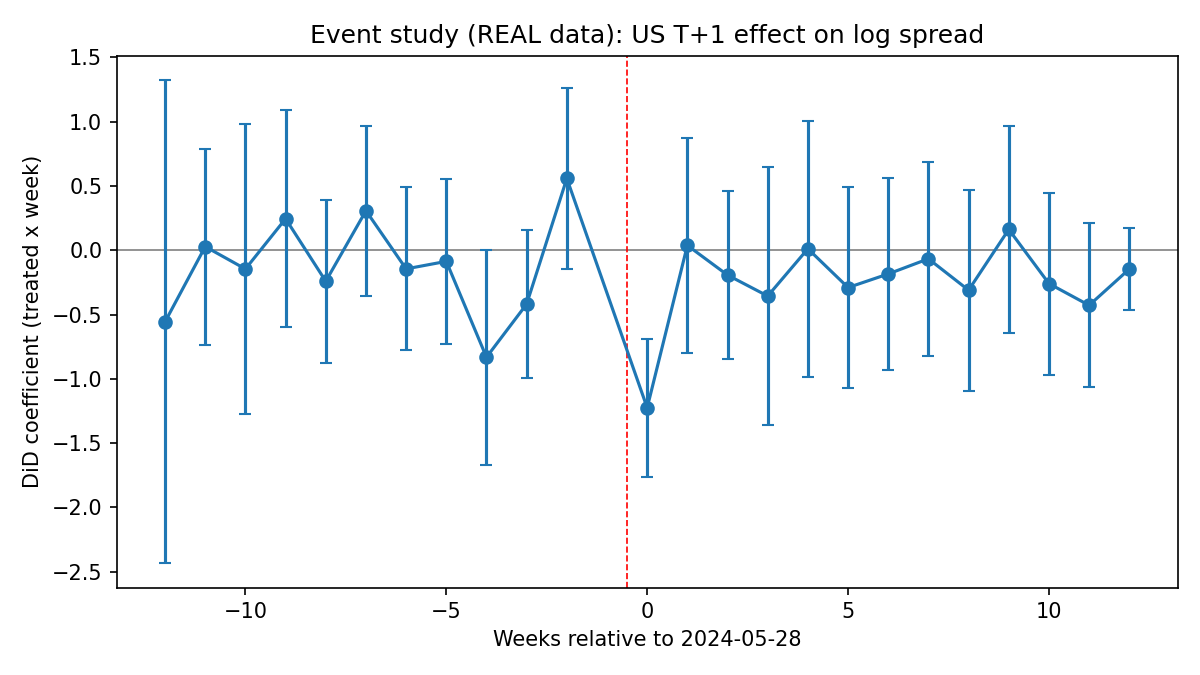
\includegraphics[width=.82\textwidth]{eventstudy_REAL.png}}{\fbox{Upload eventstudy\_REAL.png to display the event-study figure}}
\caption{Event study: weekly DiD coefficients for the log spread around 28 May 2024
(week $-1$ omitted). Flat leads support parallel trends; post-event coefficients
fluctuate around zero, consistent with the imprecise null.}
\label{fig:es}
\end{figure}

\section{Robustness}\label{sec:robust}
Table~\ref{tab:robust} collects the spread and volatility coefficients across every specification.

\begin{table}[h]\centering
\caption{Robustness: the coefficient of interest across specifications}
\label{tab:robust}
\begin{tabular}{lccccc}
\toprule
 & \multicolumn{2}{c}{ln(spread)} & \multicolumn{2}{c}{ln(volatility)} & \\
\cmidrule(lr){2-3}\cmidrule(lr){4-5}
Specification (sample) & $\beta$ & (SE) & $\beta$ & (SE) & Clusters \\
\midrule
Main: 19 cross-listed pairs         & 0.010  & (0.289) & $-$0.198 & (0.031) & 19 \\
Pair-gap (US$-$home), firm FE       & 0.016  & (0.286) & $-$0.193 & (0.031) & 19 \\
Weekly aggregation                  & $-$0.006 & (0.283) & $-$0.186 & (0.031) & 19 \\
Non-cross-listed US vs.\ EU         & 0.133  & (0.261) & $+$0.120 & (0.036) & 23 \\
Placebo event (pre-period only)     & 0.175  & (0.210) & $+$0.175 & (0.070) & 19 \\
8-pair exploratory sample           & $-$1.050 & (0.374) & $-$0.207 & (0.063) & 8 \\
\bottomrule
\end{tabular}
\caption*{\footnotesize The spread effect is insignificant in every credible
specification; the only ``significant'' spread is the discredited 8-cluster
sample. The volatility coefficient is negative in the cross-listed samples but
positive in the non-cross-listed sample and significant under the placebo,
i.e.\ not a causal effect of T+1. Standard errors clustered by firm.}
\end{table}

\textbf{Sample size at the cluster level.} An initial sample of only 8 cross-listed
pairs produced a large, ``significant'' spread coefficient ($-1.05$, $t=-2.8$),
implying an implausible 65\% spread reduction. Expanding to 19 pairs collapses it
to zero. With 8 clusters, cluster-robust inference is unreliable and a noisy proxy
produced a spurious effect---an instance of the few-cluster problem
flagged in Section~2.

\textbf{Weekly aggregation.} Daily US and European closes are one session apart, so
$\delta_t$ pairs slightly different information sets. Averaging each listing's
outcomes to the ISO-week level and re-estimating \eqref{eq:did} leaves the spread
null intact ($\beta=-0.006$, SE $0.283$), so the result is not an artifact of the
time-zone mismatch.

\textbf{An independent control group.} The within-pair design's
main vulnerability is that arbitrage links the two lines, so the home ``control''
may be partly treated. I therefore re-run the DiD on stocks that share no arbitrage book: 12 US-only large caps (treated) versus 11 UK/EU-only large caps
(control). The spread DiD is $+0.133$ (SE $0.261$, $t=0.51$)---again null. Two designs with very different spillover exposure agree, so the null is unlikely to be a SUTVA artifact.

\textbf{Robustness of inference to the cluster count.} Because cluster-robust
standard errors with 19 clusters rest on large-$G$ asymptotics and can over-reject,
I do not rest the conclusion on any single specification's standard error. The transaction-cost null recurs in a different sample
with a different clustering structure (the 23 non-cross-listed firms above) and
under weekly aggregation. A conclusion that holds across independent samples does
not depend on the 19-cluster asymptotics; this corroboration substitutes for the wild cluster bootstrap noted in Section~2. With only 19
clusters the cluster-robust standard errors are, if anything, biased downward, so the true confidence interval is likely even wider than the
reported $[-0.56,0.58]$, strengthening the imprecision point. As a check matching the within-pair estimand
directly, the pair-gap specification (Table~\ref{tab:robust}, row 2)---the
US-minus-home spread gap regressed on Post with firm fixed effects---gives
$\beta=0.016$ (SE $0.286$), substantively identical to the main estimate.

\textbf{Why the volatility result is not causal.} Two checks sink it. First, a
pre-period placebo (a fake event on 2 April 2024, using only pre-event data) yields
a significant volatility coefficient ($+0.175$, $t=2.5$): treated-line
volatility was already diverging from control before any policy change, violating
parallel trends for that outcome. Second, in the non-cross-listed sample the
volatility DiD is $+0.120$ ($t=3.3$)---the opposite sign to the cross-listed
$-0.198$. A coefficient that flips sign with the control group and fails its
placebo is more consistent with a differential US-versus-Europe trend than with an effect of T+1. The spread
null, by contrast, passes its placebo ($+0.175$, $t=0.83$, insignificant) and holds
across both samples.

\section{Conclusion}
I asked whether compressing the equity settlement cycle improves market quality,
using the 2024 US move to T+1 and a within-firm cross-listing design. For transaction costs, I find a bounded null: the spread effect is
statistically insignificant, and although the confidence interval is too wide to
call it a tight zero, the absence of any effect is consistent across weekly
aggregation and across an independent non-cross-listed control group. The large
volatility decline that first appeared does not survive a placebo test or a change
of control group, so I decline to read it causally. Substantively, the shorter cycle shows no detectable deterioration in trading costs, which is reassuring for the policy, though the data cannot rule out moderate effects. Methodologically, the
project taught two lessons the hard way: inference credibility is governed by the
number of \emph{clusters}, not observations (my first ``significant'' result was an
artifact of eight clusters), and placebo plus alternative-control tests help separate a causal estimate from a trend. Sharper estimates would need intraday quote data (e.g., TAQ), and India's parallel T+0 move of March 2024 offers a natural external-validity check.

\appendix
\section*{Appendix A: Data construction}
Each listing's series is daily open, high, low, close, and volume from Yahoo
Finance (2 Jan--30 Sep 2024), pulled by ticker (US lines have no suffix; home
lines carry exchange suffixes, e.g.\ \texttt{.L} London, \texttt{.DE} Frankfurt,
\texttt{.PA} Paris, \texttt{.SW} Zurich). Because every outcome is a within-listing ratio or log change---the Corwin--Schultz spread is a function of the
high/low ratio, Amihud is $|$return$|$ per dollar volume, Parkinson uses
$\ln(H/L)$---the cross-currency price levels of the US and home lines do not enter,
and any ADR-to-ordinary share ratio is a fixed scale factor absorbed by the listing
fixed effect. Days with a missing OHLC field are dropped. Logs add a small constant
($10^{-6}$ for the spread, which the Corwin--Schultz estimator truncates at zero;
$10^{-9}$ for volatility) to handle exact zeros. I do not winsorize in the baseline (a possible extension); the 8-pair-vs-19-pair comparison suggests the estimates are not driven by outliers or by particular firms once the sample is adequately sized.

\section*{Appendix B: Estimation commands}
All estimates are OLS with two-way fixed effects and firm-level cluster-robust
standard errors. The reported
numbers were generated with the following Stata commands:

\begin{verbatim}
* main DiD, e.g. for the spread (Table 2):
reg ln_spread treatpost i.ticker i.date, vce(cluster firm)
* equivalent fixed-effects form:
xtreg ln_spread treatpost i.date, fe vce(cluster firm)
* event study (Figure 2): interact treat with event-week dummies
xtreg ln_spread ib(-1).relweek#i.treat i.date, fe vce(cluster firm)
testparm i(0/12).relweek#i.treat
* weekly robustness: collapse to firm-listing-week means, then re-run the DiD
* triangulation: same DiD on non-cross-listed US (treat=1) vs EU (treat=0) stocks
\end{verbatim}


\section*{References}
\quad  Amihud, Y. (2002). Illiquidity and stock returns. 

\textit{J. Financial Markets}.
Baig, A., et al.\ (2022). Settling down: T+2 settlement cycle and liquidity.

\textit{European Financial Management}.
Cameron, A.C., Gelbach, J., \& Miller, D. (2008). Bootstrap-based improvements for
inference with clustered errors. 

\textit{Rev. Economics and Statistics}.
Corwin, S., \& Schultz, P. (2012). A simple way to estimate bid-ask spreads from
daily high and low prices. 

\textit{J. Finance}.
Goodman-Bacon, A. (2021). Difference-in-differences with variation in treatment
timing. 

\textit{J. Econometrics}.
Parkinson, M. (1980). The extreme value method for estimating the variance of the
rate of return. 

\textit{J. Business}.
SEC (2023). Shortening the securities transaction settlement cycle.

\end{document}
